\documentclass[tikz,border=6pt]{standalone}
% Shared style for the HERMESS schematic figures (compiled by build.sh).
% ETH palette; Latin Modern (the LaTeX default) to match the documentation.
\usepackage{amsmath}
\usepackage{tikz}
\usetikzlibrary{arrows.meta,positioning,calc,shapes.geometric,circuits.ee.IEC}
\definecolor{ethblue}{HTML}{215CAF}
\definecolor{ethpetrol}{HTML}{007894}
\definecolor{ethgrey}{HTML}{6F6F6F}
\tikzset{
  block/.style      = {draw=ethblue, thick, fill=ethblue!8, minimum height=9mm,
                       minimum width=16mm, inner sep=2.5pt, align=center},
  sum/.style        = {draw=ethblue, thick, circle, fill=white, minimum size=4.5mm, inner sep=0pt},
  sig/.style        = {-{Latex[length=2.4mm]}, thick},
  wire/.style       = {thick},
  node distance     = 9mm and 12mm,
  every node/.style = {font=\small},
  lbl/.style        = {font=\small, inner sep=1.5pt},
  port/.style       = {font=\small\itshape, text=ethgrey},
}

\begin{document}
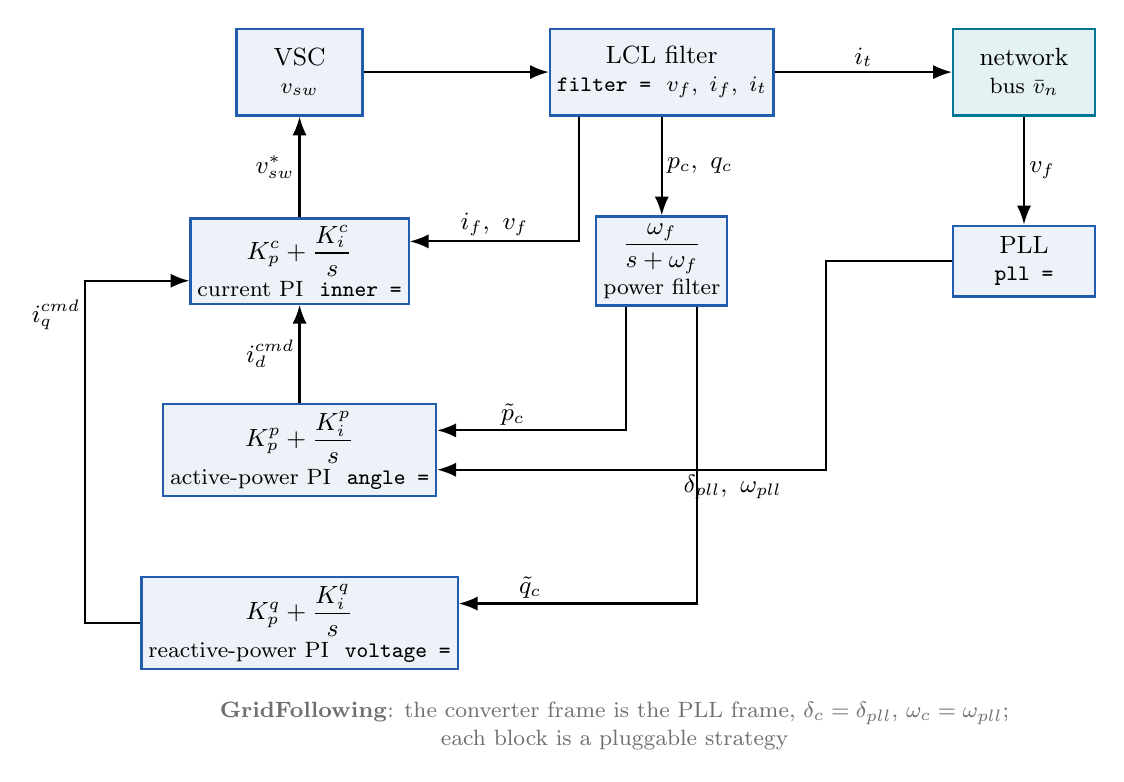
\begin{tikzpicture}[x=1cm,y=1cm]
  % power path (identical to the voltage-mode figure)
  \node[block, minimum width=16mm, minimum height=11mm] (vsc) at (0,0) {VSC\\[-1pt]{\footnotesize $v_{sw}$}};
  \node[block, minimum width=26mm, minimum height=11mm] (lcl) at (4.6,0) {LCL filter\\[-1pt]{\footnotesize\texttt{filter =}\ \ $v_f,\ i_f,\ i_t$}};
  \node[block, minimum width=18mm, minimum height=11mm, fill=ethpetrol!10, draw=ethpetrol] (grid) at (9.2,0) {network\\[-1pt]{\footnotesize bus $\bar v_n$}};
  \draw[sig] (vsc) -- (lcl);
  \draw[sig] (lcl) -- (grid) node[midway, above, lbl] {$i_t$};
  % measurement filter (narrower than the LCL block, so the feedback tap on
  % the LCL underside drops past its left edge)
  \node[block, minimum width=16mm] (meas) at (4.6,-2.4) {$\dfrac{\omega_f}{s + \omega_f}$\\[1pt]{\footnotesize power filter}};
  \draw[sig] (lcl) -- (meas) node[midway, right, lbl] {$p_c,\ q_c$};
  % current-mode inner loop
  \node[block, minimum width=24mm] (inner) at (0,-2.4) {$K_p^{c} + \dfrac{K_i^{c}}{s}$\\[1pt]{\footnotesize current PI\ \ \texttt{inner =}}};
  \draw[sig] (inner) -- (vsc) node[midway, left, lbl] {$v_{sw}^{*}$};
  \draw[sig] ($(lcl.south)+(-1.05,0)$) |- ($(inner.east)+(0,0.25)$) node[pos=0.75, above, lbl] {$i_f,\ v_f$};
  % power PI outers
  \node[block, minimum width=24mm] (ppi) at (0,-4.8) {$K_p^{p} + \dfrac{K_i^{p}}{s}$\\[1pt]{\footnotesize active-power PI\ \ \texttt{angle =}}};
  \node[block, minimum width=24mm] (qpi) at (0,-7.0) {$K_p^{q} + \dfrac{K_i^{q}}{s}$\\[1pt]{\footnotesize reactive-power PI\ \ \texttt{voltage =}}};
  \draw[sig] (ppi) -- (inner) node[midway, left, lbl] {$i_d^{cmd}$};
  \draw[sig] (qpi.west) -- ++(-0.7,0) |- ($(inner.west)+(0,-0.25)$) node[pos=0.45, left, lbl] {$i_q^{cmd}$};
  \draw[sig] ($(meas.south)+(-0.45,0)$) |- ($(ppi.east)+(0,0.25)$) node[pos=0.8, above, lbl] {$\tilde p_c$};
  \draw[sig] ($(meas.south)+(0.45,0)$) |- ($(qpi.east)+(0,0.25)$) node[pos=0.85, above, lbl] {$\tilde q_c$};
  % the PLL sits directly under the network block and fixes the frame
  \node[block, minimum width=18mm] (pll) at (9.2,-2.4) {PLL\\[-1pt]{\footnotesize\texttt{pll =}}};
  \draw[sig] (grid) -- (pll) node[midway, right, lbl] {$v_f$};
  \draw[sig] (pll.west) -- ++(-1.6,0) |- ($(ppi.east)+(0,-0.25)$) node[pos=0.62, below, lbl] {$\delta_{pll},\ \omega_{pll}$};
  \node[lbl, text=ethgrey, align=center] at (4.0,-8.3)
    {\footnotesize \textbf{GridFollowing}: the converter frame is the PLL frame, $\delta_c = \delta_{pll}$, $\omega_c = \omega_{pll}$;\\[-1pt]
     \footnotesize each block is a pluggable strategy};
\end{tikzpicture}
\end{document}
